\documentclass[11pt, addpoints, answers]{exam}

\usepackage[utf8]{inputenc}
\usepackage[T1]{fontenc}
\usepackage[margin  = 1in]{geometry}
\usepackage{amsmath, amscd, amssymb, amsthm, verbatim}
\usepackage{mathabx}
\usepackage{setspace}
\usepackage{float}
\usepackage{color}
\usepackage{graphicx}   
\usepackage[colorlinks=true]{hyperref}
\usepackage{tikz}

\usetikzlibrary{shapes,arrows}
%%%<
\usepackage{verbatim}
%%%>
\usetikzlibrary{automata,arrows,positioning,calc}

\usetikzlibrary{trees}

\shadedsolutions
\definecolor{SolutionColor}{RGB}{214,240,234}

\newcommand{\bbC}{{\mathbb C}}
\newcommand{\R}{\mathbb{R}}            % real numbers
\newcommand{\bbR}{{\mathbb R}}
\newcommand{\Z}{\mathbb{Z}}            % integers
\newcommand{\bbZ}{{\mathbb Z}}
\newcommand{\bx}{\mathbf x}            % boldface x
\newcommand{\by}{\mathbf y}            % boldface y
\newcommand{\bz}{\mathbf z}            % boldface z
\newcommand{\bn}{\mathbf n}            % boldface n
\newcommand{\br}{\mathbf r}            % boldface r
\newcommand{\bc}{\mathbf c}            % boldface c
\newcommand{\be}{\mathbf e}            % boldface e
\newcommand{\bE}{\mathbb E}            % blackboard E
\newcommand{\bP}{\mathbb P}            % blackboard P

\newcommand{\ve}{\varepsilon}          % varepsilon
\newcommand{\avg}[1]{\left< #1 \right>} % for average
%\renewcommand{\vec}[1]{\mathbf{#1}} % bold vectors
\newcommand{\grad}{\nabla }
\newcommand{\lb}{\langle }
\newcommand{\rb}{\rangle }

\def\Bin{\operatorname{Bin}}
\def\Var{\operatorname{Var}}
\def\Geom{\operatorname{Geom}}
\def\Pois{\operatorname{Pois}}
\def\Exp{\operatorname{Exp}}
\newcommand{\Ber}{\operatorname{Ber}}
\def\Unif{\operatorname{Unif}}
\def\No{\operatorname{N}}
\newcommand{\E}{\mathbb E}            % blackboard E
\def\th{\theta }            % theta shortcut
\def\V{\operatorname{Var}}
\def\Var{\operatorname{Var}}
\def\Cov{\operatorname{Cov}}
\def\Corr{\operatorname{Corr}}
\newcommand{\epsi}{\varepsilon}            % epsilon shortcut

\providecommand{\norm}[1]{\left\lVert#1\right\rVert} %norm
\providecommand{\abs}[1]{\left \lvert#1\right \rvert} %absolute value

\DeclareMathOperator{\lcm}{lcm}
\newcommand{\ds}{\displaystyle}	% displaystyle shortcut

\def\semester{2021-2022}
\def\course{Modèles Aléatoires Discrets}
\def\title{\MakeUppercase{Examen de Deuxième Session}}
\def\name{Pierre-O Goffard}
%\def\name{Professor Wildman}

\setlength\parindent{0pt}

\cellwidth{.35in} %sets the minimum width of the blank cells to length
\gradetablestretch{2.5}

%\bracketedpoints
%\pointsinmargin
%\pointsinrightmargin

\begin{document}


\runningheader{\course  \vspace*{.25in}}{}{\title \vspace*{.25in}}
%\runningheadrule
\runningfooter{}{Page \thepage\ of \numpages}{}

% \firstpageheader{Name:\enspace\hbox to 2.5in{\hrulefill}\\  \vspace*{2em} Section: (circle one) TR: 3-3:50 \textbar\, TR: 5-5:50 \textbar\,  TR: 6-6:50(Xu) \textbar\,  TR: 6-6:50 }{}{Perm \#: \enspace\hbox to 1.5in{\hrulefill}\\ \vspace*{2em} Score:\enspace\hbox to .6in{\hrulefill} $/$\numpoints}
\extraheadheight{.25in}

\hrulefill

\vspace*{1em}

% Heading
{\center \textsc{\Large\title}\\
	\vspace*{1em}
	\course -- \semester\\
	Pierre-O Goffard\\
}
\vspace*{1em}

\hrulefill

\vspace*{2em}

\noindent {\bf\em Instructions:} On éteint et on range son téléphone.
\begin{itemize}
	\item La calculatrice et les appareils éléctroniques ne sont pas autorisés.
	\item Vous devez justifier vos réponses de manière claire et concise.
	\item Vous devez écrire de la manière la plus lisible possible. Souligner ou encadrer votre réponse finale.
	\item \underline{Document autorisé:} Une feuille manuscrite recto-verso

\end{itemize}


\begin{center}
	\gradetable[h]
\end{center}

\smallskip

\begin{questions}
\question Soit deux joueurs $A$ et $B$ engagés dans un jeu. Initialement, les deux joueurs sont à égalité, la victoire revient au joueur qui parvient à gagner deux parties successivement. Le temps est indicé sur chaque partie et l'état du jeu est modélisé par une chaine de Markov $(X_n)_{n\geq0}$ à $5$ états avec 
\begin{itemize}
	\item Etat 1: \textit{Egalité} (E)
	\item Etat 2: \textit{Avantage A} (AvA)
	\item Etat 3: \textit{Avantage B} (AvB)
  \item Etat 4: \textit{Victoire A} (VA)
	\item Etat 5: \textit{Victoire B} (VB)
\end{itemize}
La probabilité que $A$ remporte une manche est égale à $3/5$ (celle de B est donc $2/5$) et on suppose que $X_0 = E$. Une trajectoire possible du processus est par exemple $E-AvA-E-AvA-VA$, cela signifie que $A$ a remporté la première partie puis $B$ a remporté la deuxième (remettant les deux joueurs à égalité) puis $A$ a gagné les deux parties suivantes le menant à la victoire. La victoire de l'un des deux joueurs entrainent l'arrêt du jeu.
\begin{parts}
\part[2] Donner le graph et la matrice des transitions de $(X_n)_{n\geq0}$
\begin{solution}
\begin{center}
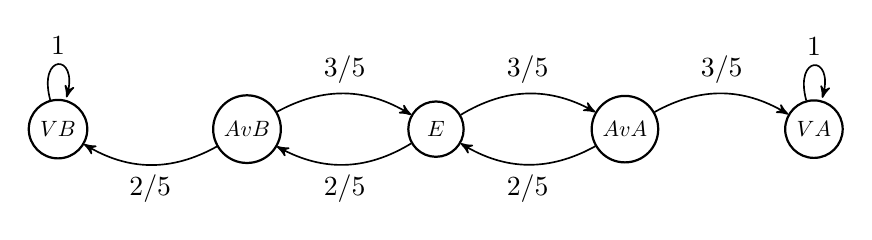
\begin{tikzpicture}[->, >=stealth', auto, semithick, node distance=3cm]
\tikzstyle{every state}=[fill=white,draw=black,thick,text=black,scale=0.8]
\node[state]    (1)                     {$E$};
\node[state]    (2)[right of=1]   {$AvA$};
\node[state]    (3)[left of=1]   {$AvB$};
\node[state]    (4)[right of=2]   {$VA$};
\node[state]    (5)[left of=3]   {$VB$};
\path
(1) edge[bend left]     node{$3/5$}         (2)
(1) edge[bend left]     node{$2/5$}         (3)

(2) edge[bend left]      node{$3/5$}      (4)
    edge[bend left]     node{$2/5$}      (1)
(3) edge[bend left]      node{$3/5$}     (1)
    edge[bend left]     node{$2/5$}      (5)
(4) edge[loop above]      node{$1$}     (4)
(5) edge[loop above]      node{$1$}     (5);


\end{tikzpicture}
\end{center}
$$
Q = \left(\begin{array}{ccccc}
0&3/5&2/5&0&0\\
2/5&0&0&3/5&0\\
3/5&0&0&0&2/5\\
0&0&0&1&0\\
0&0&0&0&1\end{array}\right)
$$
\end{solution}
\part[3] Donner les classes de communications de $(X_n)_{n\geq0}$. Sont-elles ouvertes ou fermées? La chaine $(X_n)_{n\geq0}$ est-elle irréductible?
\begin{solution}
$3$ classes de communications 
\begin{itemize}
	\item $\{E, AvA, AvB\}$ est ouverte
	\item $\{VA\}$ et $\{VB\}$ sont fermées
\end{itemize}
$(X_n)_{n\geq0}$ n'est pas irréductible.
\end{solution}
\part[2] Calculer la durée (le nombre de partie à jouer) moyenne du jeu sachant que $X_0 = E$.\\

\underline{Indication:} Introduire le temps d'arrêt
$$
\tau = \inf \{n\geq0\text{ : }X_n\in\{VA,VB\}\},
$$
et calculer l'espérance 
$$
\mathbb{E}_E(\tau) = \mathbb{E}(\tau|X_0 = E),
$$
via l'analyse à un pas.
\begin{solution}
Soit le temps d'arrêt
$$
\tau = \inf\{n\geq0\text{ ; }X_n\in\{VA, VB\}\}
$$
On a $\mathbb{E}_{VA}(\tau) = \mathbb{E}_{VG}(\tau) = 0$ et en utilisant l'analyse à un pas
$$
\begin{cases}
\mathbb{E}_{E}(\tau)=1 + \frac{3}{5}\mathbb{E}_{AvA}(\tau)+\frac{2}{5}\mathbb{E}_{AvB}(\tau)\\
\mathbb{E}_{AvA}(\tau)=1 + \frac{2}{5}\mathbb{E}_{E}(\tau)\\
\mathbb{E}_{AvB}(\tau)=1 + \frac{3}{5}\mathbb{E}_{E}(\tau)\\
\end{cases}
$$
Il vient donc, après resolution du système $E_E(\tau)=50/13$.
\end{solution}
\part[2] Calculer la probabilité que $A$ remporte le jeu sachant que $X_0 = E$.
\begin{solution}
On utilise l'analyse à un pas. Soit l'évènement $VA =\text{ "Le joueur A remporte le jeu"}$, on a 
$$
\mathbb{P}_{VA}(VA) = 1\text{ et }\mathbb{P}_{VB}(VA) = 0
$$
La résolution du système 
$$
\begin{cases}
\mathbb{P}_{E}(VA)= \frac{3}{5}\mathbb{P}_{AvA}(VA)+\frac{2}{5}\mathbb{P}_{AvB}(VA)\\
\mathbb{P}_{AvA}(VA)= \frac{2}{5}\mathbb{P}_{E}(VA)+ \frac{3}{5}\\
\mathbb{P}_{AvB}(VA)= \frac{3}{5}\mathbb{P}_{E}(VA)\\
\end{cases}
$$
donne $\mathbb{P}_{E}(VA) = 9/13$.
\end{solution}
\end{parts} 
\question Soit $(N_t)_{t\geq 0}$ un processus de Poisson d'intensité $\lambda>0$. Soit le processus $(X_t)_{t\geq0}$ défini par 
$$
X_t = X_0(-1)^{N_t}, \text{ }t\geq 0,
$$ 
où $X_0$ est une variable aléatoire d'espérance $\mu$ et de variance $\sigma^2$, indépendante de $(N_t)_{t\geq0}$.\\
\underline{Rappel:} La covariance de deux variables aléatoires $X$ et $Y$ est donnée par 
$$
\text{Cov}(X,Y) =\mathbb{E}\left[(X-\mathbb{E}(X))(Y-\mathbb{E}(Y))\right] = \mathbb{E}(XY) -\mathbb{E}(X)\mathbb{E}(Y) .
$$
\begin{parts}
% \part[1] Calculer $\text{Cov}(N_t, N_s)$ pour $t,s\geq0$, en fonction de $t,s$ et $\lambda$.
% \begin{solution}
% $\text{Cov}(N_t, N_s) = \lambda\min(s,t)$.
% \end{solution}
\part[2] Calculer $\mathbb{E}(X_t)$ et $\mathbb{V}(X_t)$  en fonction de $\mu, \lambda,$ et $t$.
\begin{solution}
$\mathbb{E}(X_t) = \mu e^{-2\lambda t}$ et $\mathbb{V}(X_t) = \sigma^2 + \mu^2(1-e^{-4\lambda t})$.
\end{solution}
\part[1] Calculer $\text{Cov}(X_t, X_s)$ en fonction de $\mu, \sigma^2, \lambda,$ et $t$.
\begin{solution}
$\text{Cov}(X_t, X_s) = (\sigma^2 +\mu^2) e^{-2\lambda |t-s|}- \mu^2 e^{-2\lambda (t+s)}$.
\end{solution}
\end{parts}
\question Soit $p\in [0,1]$ et $q = 1-p$. Soit la chaine de Markov $(X_n)_{n\geq0}$ sur l'espace d'état $E = \{0, \ldots, N\}$, avec $N\in\mathbb{N}$ et de graph des transitions
\begin{center}
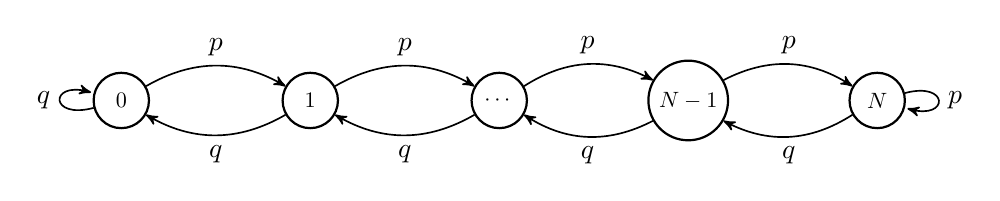
\begin{tikzpicture}[->, >=stealth', auto, semithick, node distance=3cm]
\tikzstyle{every state}=[fill=white,draw=black,thick,text=black,scale=0.8]
\node[state]    (1)                     {$0$};
\node[state]    (2)[right of=1]   {$1$};
\node[state]    (3)[right of=2]   {$\cdots$};
\node[state]    (4)[right of=3]   {$N-1$};
\node[state]    (5)[right of=4]   {$N$};
\path
(1) edge[bend left]     node{$p$}         (2)
    edge[loop left]     node{$q$}         (1)
(2) edge[bend left]      node{$p$}      (3)
    edge[bend left]     node{$q$}      (1)
(3) edge[bend left]      node{$p$}     (4)
    edge[bend left]     node{$q$}      (2)
(4) edge[bend left]      node{$p$}     (5)
    edge[bend left]      node{$q$}     (3)
(5) edge[loop right]      node{$p$}     (5)
    edge[bend left]      node{$q$}     (4)
;
\end{tikzpicture}
\end{center}
On adopte les notations suivantes  
$$
\mathbb{P}_x(\cdot) = \mathbb{P}(\cdot|X_0 = k),\text{ et },\mathbb{P}_x(\cdot) = \mathbb{P}(\cdot|X_0 = x)$$
pour la probabilité et l'espérance conditionnelle sachant $X_0 = x$ et $x\in\{0,\ldots, N\}$.
\begin{parts}
\part[3] Pour quelles valeurs de $p$ la chaine est-elle irréductible? Quand la chaine n'est pas irréductible, combien de classes de communication? Sont-elles ouvertes ou fermées?\\
\begin{solution}
La chaine est irréductible si $p\in(0,1)$. Si $p = 0$ ou $p = 1$ alors il y a $N+1$ classes de communication. Si $p = 0$ alors $\{0\}$ est la seule classe fermée et $\{1\},\ldots\{N\}$ sont des classes ouvertes.Si $p = 1$ alors $\{N\}$ est la seule classe fermée et $\{0\},\ldots\{N-1\}$ sont des classes ouvertes.
\end{solution}

\textbf{Dans la suite on suppose que $p\in(0,1)$.}
\part[1] Soit 
$$
\tau =\inf\left\{n\geq 0 \text{ ; }X_n\in\{0, N\}\right\}
$$
et 
$$
f(x, \lambda) = \mathbb{E}_x(e^{-\lambda\tau}) , \text{ pour }\lambda\in\mathbb{R}.
$$
Donner la valeur de $f(0, \lambda)$ et $f(N, \lambda)$.
\begin{solution}
$f(0, \lambda) = f(N, \lambda) = 1$.
\end{solution}
\part[1] Exprimer $\mathbb{P}_x(\tau = n)$ en fonction de $\mathbb{P}_{x-1}(\tau = n-1)$ et $\mathbb{P}_{x+1}(\tau = n-1)$, pour $n>1$ et $x\in\{1,\ldots, N-1\}$.
\begin{solution}
Il s'agit d'une analyse à un pas, nous avons
$$
\mathbb{P}_x(\tau = n) = q\mathbb{P}_{x-1}(\tau = n-1) + p\mathbb{P}_{x+1}(\tau = n-1).
$$
\end{solution}
\part[1] En déduire que 
$$
f(x, \lambda) = e^{-\lambda}\left[qf(x-1, \lambda) + pf(x+1, \lambda)\right],
$$
pour $x\in\{1,\ldots, N-1\}$
\begin{solution}
\begin{eqnarray*}
f(x, \lambda) &=&\sum_{n = 0}^{+\infty}e^{-\lambda n}\mathbb{P}_x(\tau = n) \\
&=&\sum_{n = 1}^{+\infty}e^{-\lambda n}\mathbb{P}_x(\tau = n) \\ 
&=&\sum_{n = 1}^{+\infty}e^{-\lambda n}q\mathbb{P}_{x-1}(\tau = n-1) + p\mathbb{P}_{x+1}(\tau = n-1)\\
&=&e^{-\lambda}q\sum_{n = 0}^{+\infty}e^{-\lambda n}\mathbb{P}_{x-1}(\tau = n) + e^{-\lambda}p\sum_{n = 0}^{+\infty}e^{-\lambda n}\mathbb{P}_{x+1}(\tau = n)\\
&=&e^{-\lambda}qf(x-1, \lambda) + e^{-\lambda}pf(x+1, \lambda)
\end{eqnarray*}
\end{solution}
\part[1] Soit $g(x) = \mathbb{E}_x(\tau)$. Donner $g(0)$ et $g(N)$
\begin{solution}
$g(0) = g(N) = 0$
\end{solution} 
\part[1] On note que 
$$
g(x) = -\frac{\partial f}{\partial \lambda}(x,0).
$$ 
En déduire (en utilisant (c)) que 
$$  
g(x) = qg(x-1)+pg(x+1)+1,
$$
pour $x\in\{1,\ldots, N-1\}$.
\\
\begin{solution}
On dérive l'équation
$$
f(x, \lambda) = e^{-\lambda}\left[qf(x-1, \lambda) + pf(x+1, \lambda)\right],
$$
par rapport à $\lambda$ et on évalue pour $\lambda = 0$.
\end{solution}
\textbf{Dans la suite on suppose que $p\neq q$ et on rappelle que $q = 1-p$.}
\part[1] Trouver $c\in\mathbb{R}$ pour que $g(x) = cx$ soit une solution de l'équation
$$
g(x) = qg(x-1)+pg(x+1)+1.
$$
\begin{solution}
$c = 1/(q-p)$
\end{solution}
\part[1] Quelles sont les valeurs de $r\in\mathbb{R}$ pour lesquels la fonction $g_0(r) = r^{x}$ est solution de l'équation homogène
$$
g_0(x) = qg_0(x-1)+pg_0(x+1).
$$
\underline{Indication:} Bien remplacer $q$ par $1-p$ dans l'équation homogène.
\begin{solution}
Les valeurs de $r$ possibles sont les solutions de l'équation 
$$
pr^2-r+ 1-p=0.
$$
L'équation précédente à deux solutions réelles avec 
$$
r_1 = \frac{1-p}{p}\text{ et }r_2 = 1
$$
\end{solution}
\part[1] En déduire $E_x(\tau)$ pour $x\in\{1,\ldots, N-1\}$.
\begin{solution}
La forme générale des solutions de l'équation
$$
g(x) = qg(x-1)+pg(x+1)+1.
$$
est donnée par 
$$
g(x) = \frac{x}{q-p} + Ar_1^x+ Br_2^x.
$$
avec $A$ et $B$ des constantes que l'on identifie grâce aux conditions initiales avec $g(0) = g(N) = 0$. ON obtient finalement 
$$
g(x) = \frac{x}{q-p} + \frac{p^N}{p^N-q^N}\frac{N}{1-2p}\left[1-\left(\frac{1-p}{p}\right)^x\right].
$$
\end{solution}


\end{parts}



\end{questions}
%-------------------------------TABLE-------------------------------
\newpage
\hrule
\vspace*{.15in}
\begin{center}
  \large\MakeUppercase{Formulaire}
\end{center}
\vspace*{.15in}
\hrule
\vspace*{.25in}

\renewcommand\arraystretch{3.5}
\begin{table}[H]
\begin{center}
\footnotesize
\begin{tabular}{|c|c|c|c|c|c|}

\hline
Nom & abbrev. & Loi & $\E(X)$ & $\Var(X)$ & FGM\\
\hline\hline
Binomial & $\Bin(n,p)$ & $\binom{n}{k}p^k(1-p)^{n-k}$ & $np$ & $np(1-p)$ & $[(1-p)+pe^t]^n$\\
\hline
Poisson & $\Pois(\lambda)$ & $e^{-\lambda}\dfrac{\lambda^k}{k!}$ & $\lambda$ & $\lambda$ &$ \exp(\lambda(e^t-1))$\\
\hline
Geometric & $\Geom(p)$ & $(1-p)^{k-1}p$ & $\dfrac{1}{p}$ & $\dfrac{1-p}{p^2}$ & $\frac{pe^t}{1-(1-p)e^t}$ pour  $t<-\ln(1-p)$\\
\hline
Uniform & $\Unif(a,b)$ & $\begin{cases} \dfrac{1}{b-a} & a\leq t\leq b\\ 0 & \text{sinon}\end{cases}
$ & $\dfrac{a+b}{2}$ & $\dfrac{(b-a)^2}{12}$ & $\frac{e^{tb}-e^{ta}}{t(b-a)}$\\
\hline
Exponential & $\Exp(\lambda)$ & $\begin{cases} \lambda e^{-\lambda t} & t\geq 0 \\ 0 & t<0\end{cases}$ & $\dfrac{1}{\lambda}$ & $\dfrac{1}{\lambda^2}$ & $\frac{\lambda}{\lambda -t}$ pour $t<\lambda$\\
\hline
Normal & $\No(\mu,\sigma^2)$ & $\left(\dfrac{1}{\sqrt{2\pi\sigma^2}}\right)\operatorname{exp}{\left(\dfrac{-(t-\mu)^2}{2\sigma^2}\right)}$ & $\mu$ & $\sigma^2$ & $e^{\mu t}e^{\sigma^2t^2/2}$\\
\hline
\end{tabular}
\end{center}
\end{table}%


\end{document}